\documentclass[english]{cpp-hmwk}
   \usepackage{blindtext}

\begin{document}
\Homework{Lindenmayer systems - a C++ implementation}{Steffen Knoblauch}

\begin{abstract}
Lindenmayer Systems, short L-systems, are the result of \textbf{research from Lindenmayer et al.}\footnote{ZITIEREN} about the geometric features of plants.
L-systems are a concept to mathematicaly/formal describe and model the growth processes of plant development. They are not only restricted to the plant based developments, but can also be used to generate fractals.

L-systems start with a defined state and use rules, like a formal grammar, to transform or rather rewrite the current state to create the next state of the development or the fractal.
It is therefore possible to successive calculate each state of the development of a plant or a fractal.
Such a state of a L-system can be interpreted as commands for a turtle graphic, which creates the opportunity to draw the created fractals or plant states. 

Goal of this paper is to design an architecture for L-systems, which includes an implementation for L-systems, their creation and an interface for a turtle graphic. The interface should enable the polymorphic use of different turtle graphic implementations. 
\end{abstract}

\pagebreak
\section{Introduction}
This paper is organised in several topics, beginning with section \ref{section:lindenmayer}, which is a short introduction to the general idea,  based around object rewriting, and the grammar of L- systems.

The following sections contain a discussion about the architecture and possible implementation steps. The discussion results in a final concept for an implementation.
The final concept is realized and the code is available via my github repository.\footnote{link to my github adding}

The end of the paper includes a conclusion and an outlook for possible extension in the future.

\section{Lindenmayer systems}
\label{section:lindenmayer}
\subsection{History}
\label{section:history}
''[L-systems] were introduced in 1968 by Lindenmayer as a theoretical framwork for studying the development of simple multicellular organisms [...]''\footnote{Zitiert ausd abop Preface - Abschnitt Modeling of Plants} and were later used in computer graphics to generate visuals of organisms and fractals.

On the beginning the focus of L-systems theory was based on larger plant parts and was later on extended with new interpretations, which enabled it to represent complexer and more detailed objects.

\subsection{General idea}
The general idea of a L-system is the use of a rewriting system based on a formal grammar. The formal grammar is restricted by and based on different principles, which will be discussed in section \ref{section:grammar}.

''In general, rewriting is a technique for defining complex objects by successively replacing parts of a simple initial object using a set of rewriting rules or productions.''\footnote{Zitiert von abop Chapter 1  - 1.1 Rewriting systems}


\bigskip

TODO: Erklären was self similar und development rules sind

\bigskip


For example this concept can be used to rewrite a inital string, called axiom, with defined rewriting rules.
A simple example is the following grammar, which consits of only two nonterminals, A and B, and two production rules. 
The first rule is A\rightarrow AB, the second rule is B\rightarrow A. The arrow '\rightarrow' symbols the replacement of the object on the left with the object of the right of the arrow.
The L-system has as axiom the value 'A' and will be expanded with these rules, creating the results in figure \ref{figure:simple_lsystem}.

\begin{figure}[h!]
	\centering
	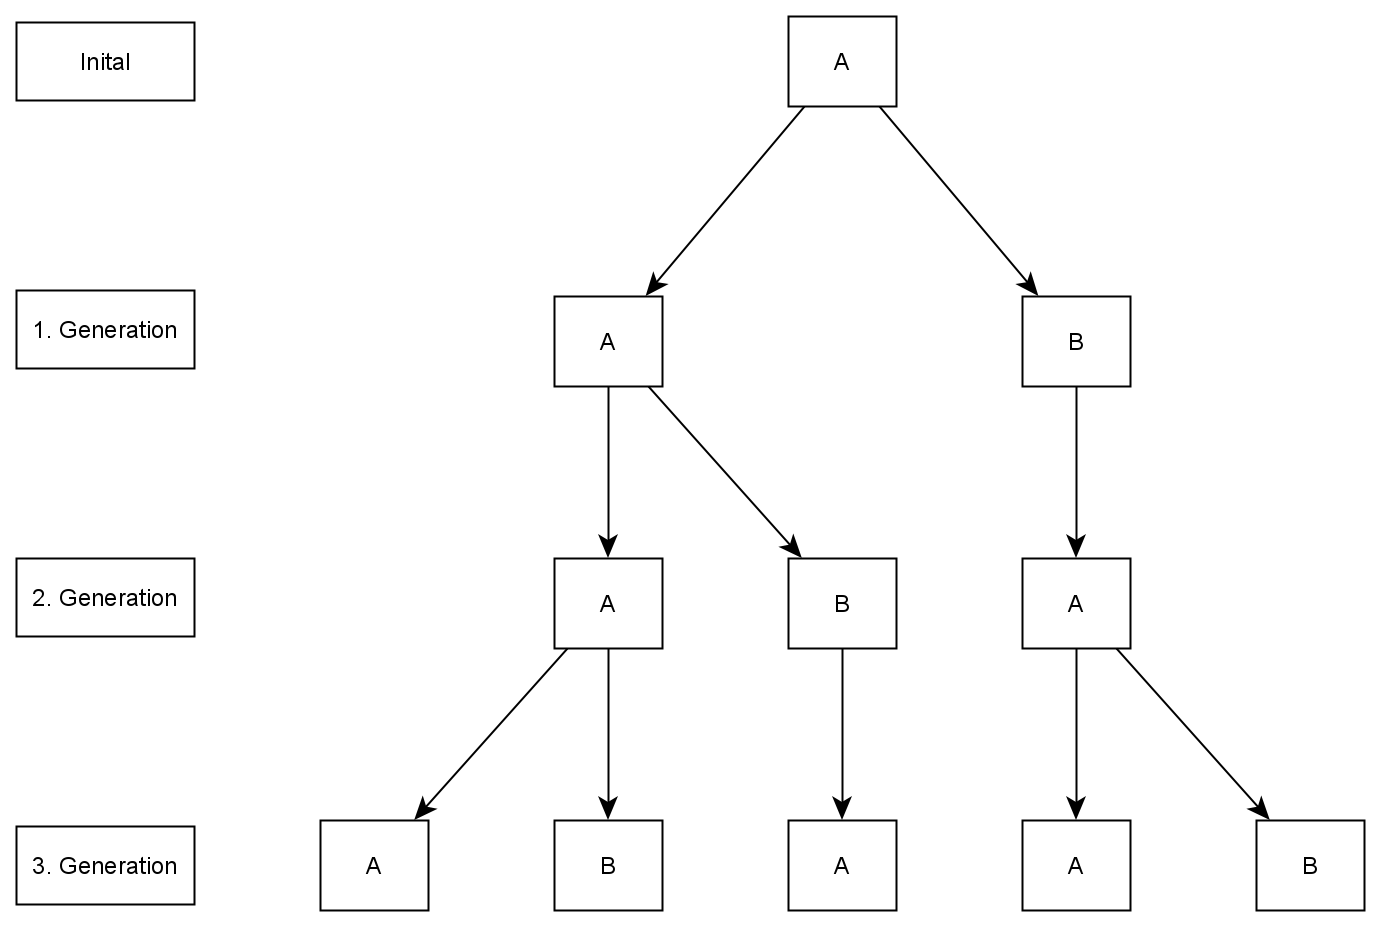
\includegraphics[width=0.7\columnwidth]{../graphs/Examples/simple_lsystem.png}
	\caption{Simple L-system}
	\label{figure:simple_lsystem}
\end{figure}

The first step is to use rule one, which replaces the nonterminal A with AB, resulting in the first generation. The result of the first generation ('AB') will be used to generate the second generation.
For all nonterminals the productions will be parallel applied. In this case the nonterminals A and B will be replaced, because both have existing production rules. This results in the second generation with 'ABA' as result.

This process can be successively repeated recursive for a arbitrary amount of generations.







\subsection{Grammar}
\label{section:grammar}
The definition of an L-system can be done similar to a Chomsky grammar, but there are some general differences. In Chomsky grammars the productions are applied sequentially, whereas in L-systems they can be applied parallel. This has some consequences for the formal properties of an L-system, for example a context-free L-system can produce a language which cannot be produced by a context-free Chomsky grammar.\footnote{Zitat abop vgl Seite 3  Abschnitt L-Systems}

\noindent This paper will only focus on a class of L-systems, the DOL-systems, which can be used for string based rewriting systems. This class is deterministic (D) and context-free (O) and can be formaly described  by a tuple:

\begin{center}
G = (V, ω, P)
\end{center}

V: set of symbols as alphabet of the l-system - consiting of terminals and non terminals

ω: axiom - nonempty word of the alphabet, which should contain at least one nonterminal

P: set of productions

\medskip
\noindent A production conistst of a predecessor, a nonterminal symbol of the alphabet, and a successor, the replacment of the nonterminal in the next generation.
To guarantee that the l-system is deterministic, there only can be one production for each nonterminal of the alphabet.The identity production is implicit a part of the set of productions.\footnote{Zitat vgl Seite 4 abop}

\bigskip

If in the process of rewriting a terminal symbol is found, there will be no explicit production applied, but rather the identity production is applied. Terminals will therefore remain in future generations and won't extend an L-system with a production.

\bigskip

\noindent As mentioned in section \ref{section:history} there are other extensions of a basic L-systems. The extensions introduce more possiblities for the generation process, like a non-deterministic behaviour. These extensions result in new grammars:

\begin{itemize}
\item Stochastic grammars: the system isn't deterministic anymore, because there can be multiple production rules for the same nonterminal with a probaility which results in a randomisation of the generation
\item Context senstive grammars: production not only look for the nonterminal, they rather look for the symbols bevor and after the current symbol to process, the context.
\item Parametric grammars: it is possible to set additional parameters for a symbol to influence the generation or the evalutaion of the data
\end{itemize}

\noindent With these new grammars it is possible to generate more complexe fractals and more detailed plant structures.

\subsection{Interpretation as turtle graphic}
The L-systems introduced to this points are capable of creating a string based on the grammar. To create a graphic of the generation of the L-system, the resulting string can be interpreted as commands of a turtle graphic.

\bigskip

WHAT IS A TURTLE GRAPHIC

\bigskip

This is based on a mapping between the symbols in the alphabet and the commands which should be called.
This could be done by an arbitrary mapping between a nonterminal or a terminal and a command. For this paper the following mapping will be used, but the concept for the architecture includes the possibility to use other mappings for the future.

\bigskip

HIER DAS MAPPING BESCHREIBEN

\bigskip




\subsection{Examples}

\begin{itemize}
	\item Koch
	\item ...
\end{itemize}
  
  


  
\pagebreak
\section{Architecture}
\begin{itemize}
	\item general focus on flexibility
	\item interfaces for future use cases
	\item different independent parts in the sample application
\end{itemize}

\section{Build System}
\begin{itemize}
	\item Cmake as buildsystem
	\item reasons why cmake
	\item problems ?
\end{itemize}



\section{FileHandler}

\begin{itemize}
	\item Load init data from file
	\item convinient way to configure the sample code
	\item no hard coded l system rules and axioms - use of the data in other apllications
\end{itemize}

\section{LSystemHandler}

\begin{itemize}
	\item Suksessiver aufbau des L Systems
	\item Nutzung von beliebiger datenstruktur mit speziellen eigenschaften -> Semantische Schnittstelle
	\item Bekommt die Daten aus dem FileHandler, kann aber aus allem kommen - belieib in andere Sachen einbindbar
\end{itemize}

\section{LSystem Datastructure}

\begin{itemize}
	\item Tree like sturcture
	\item save data not double only save pointers to the data
	\item provides access to the data with an iterator
\end{itemize}

\section{Parser for the lsystem}
\begin{itemize}
	\item Parses the result of the l system
	\item calls the Turtle Graphic on the fly
	
	\item Problem for now -> not very flexible (perhaps for the future: provide which function to call for which object)
\end{itemize}

\section{TurtleGraphic}
\subsection{Abstract class}
\subsection{TestTurtle}
\subsection{CairoTurtle}
\subsection{Further implementations}
SVG implementation
\section{Tests}
   \pagebreak
   \section{Problems and Restrictions}
   \section{Outlook}
   \footnote{\fullcite{prusinkiewiczp.lindenmayera.2004}}
\end{document}